\documentclass[12pt]{article}
\usepackage[english]{babel}
\usepackage{natbib}
\usepackage{url}
\usepackage[utf8]{inputenc}
\usepackage{amsmath}
\usepackage{amssymb}
\usepackage{graphicx}
\usepackage{parskip}
\usepackage{fancyhdr}
\usepackage{vmargin}
\usepackage{booktabs}
\usepackage[table,xcdraw]{xcolor}
\usepackage{tabularx}
\usepackage{caption} 
\usepackage{float}
\usepackage{longtable}
\usepackage{array}
\usepackage{caption}
\usepackage{subcaption}

\setmarginsrb{3 cm}{1 cm}{3 cm}{1 cm}{1 cm}{1.5 cm}{1 cm}{1.5 cm}

\newcolumntype{L}[1]{>{\raggedright\let\newline\\\arraybackslash\hspace{0pt}}m{#1}}
\newcolumntype{C}[1]{>{\centering\let\newline\\\arraybackslash\hspace{0pt}}m{#1}}
\newcolumntype{R}[1]{>{\raggedleft\let\newline\\\arraybackslash\hspace{0pt}}m{#1}}

\usepackage{natbib}

\title{Assignment \#1 - Parameter Estimation}
\date{\today}

\makeatletter
\let\thetitle\@title
\let\thesubtitle\@subtitle
\let\theauthor\@author
\let\thedate\@date
\makeatother

\pagestyle{plain}

\captionsetup[table]{skip=5pt}


\begin{document}

%%%%%%%%%%%%%%%%%%%%%%%%%%%%%%%%%%%%%%%%%%%%%%%%%%%%%%%%%%%%%%%%%%%%%%%%%%%%%%%%%%%%%%%%%

\begin{titlepage}
	\centering
    \textsc{\LARGE University of Coimbra}\\[1.0 cm]
	\textsc{\large Doctoral Program in Information Science and Technology}\\[0.5 cm]
    \textsc{\large Real Time Learning in Intelligent Systems}\\[5 cm]
	\rule{\linewidth}{0.2 mm} \\[0.4 cm]
	{ \LARGE \bfseries \thetitle}\\ [0.2 cm]
    \rule{\linewidth}{0.2 mm} \\[3 cm]
    
    \textsc{Joaquim Pedro Bento Gonçalves Pratas Leitão - 2011150072}\\[5 cm]
	
	{\large \thedate}\\[2 cm]
 
	\vfill
	
\end{titlepage}

%%%%%%%%%%%%%%%%%%%%%%%%%%%%%%%%%%%%%%%%%%%%%%%%%%%%%%%%%%%%%%%%%%%%%%%%%%%%%%%%%%%%%%%%%

\section{Introduction}
\label{introduction}

The current assignment proposes a recursive identification of two distinct linear systems. The first system is described by an \emph{ARX} model, while an \emph{ARMAX} model represents the second system.

The recursive identification task will be based on provided datasets, where inputs and corresponding outputs for the systems in question were collected and stored: for the first system, two distinct datasets were collected each containing an input and output signal over a period of time; in the second system only a single dataset was provided, containing an input signal and the corresponding response of the system.

Based on the provided datasets, the parameters of the models that describe each system can be estimated and, consequently, the corresponding linear systems can be identified. Section \ref{arx_estimation} covers the estimation procedure for the parameters of the first model, while section \ref{armax_estimation} is related with the equivalent procedure, applied for the second system. Finally, section \ref{conclusion} presents some concluding remarks.

\section{ARX Estimation}
\label{arx_estimation}

The current section covers the estimation of the parameters of the first system considered in this work, described by an \emph{ARX} model. Subsection \ref{theory_arx} provides a theoretical introduction to this task, while subsection \ref{parameter_estimation_arx} details the implementation.

\subsection{Theory}
\label{theory_arx}

In a simplistic view, a system can be considered as an object in which variables of different natures interact and produce output signals. The system can also be affected by external stimuli, which can be of two kinds: \emph{inputs}, if they can be manipulated by the observer; or \emph{disturbances}, if they cannot. A model of a system describes and represents the system in question by detailing the existing relationship between its observed signals, disturbances and outputs.

A system described by an \emph{ARX} model is assumed to be composed of two distinct components: A \emph{deterministic} and a \emph{non-deterministic} component. Figure \ref{arx_model} presents such a model. A system of this nature considers a noise filter transfer function, described by $S_{e}$, and a system transfer function described by $S_{d}$.

\begin{figure}[h]
	\centering
	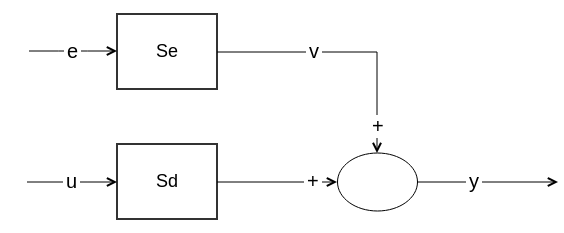
\includegraphics[scale=0.4]{images/arx_model.png}
	\caption{ARX Model.}
	\label{arx_model}
\end{figure}

In a system described by an \emph{ARX} model, the transfer function $S_{d}$ has the form $\frac{B(q)}{A(q)}$ and the noise filter has the form $\frac{1}{A(q)}$ where $A(q)$ and $B(q)$ are polynomials of the form: $A(q) = 1 + q^{-1} \times a_{1} + ... + q^{-na} \times a_{na}$ and $B(q) = q^{-1} \times b_{1} + ... + q^{-nb} \times b_{nb}$.

Therefore, the system's output is described by:

$$y_{k} = \frac{B(q)}{A(q)} u_{k} + \frac{1}{A(q)} e_{k} $$

The process of estimating the parameters of a system described by an \emph{ARX} model consists in deriving sounding estimates for the parameters $a_{1}, ... , a_{na}$ and $b_{1}, ... , b_{nb}$. A general and simplistic approach for computing these estimations comprises the following steps:

\begin{enumerate}
	\item Obtain the number of parameters, $n_{a}$ and $n_{b}$. If the values of $n_{a}$ and $n_{b}$ are unknown then they must be estimated, using expert knowledge of the system's behaviour and historical information of its inputs and outputs.
	
	\item Compute the estimations of the parameters using a recursive algorithm:
	\begin{enumerate}
		\item Consider the disturbance, $e_{k}$, to be null (that is, equal to 0) for all time instances. The reason for this assumption has to due with the fact that the disturbance is assumed to be random, following a Gaussian distribution with mean equal to 0. As only input and output information is available, it is impossible to draw any assumption about $e_{k}$. As such, it is common to consider its most probable value, that is, 0.
		
		\item Define a forgetting factor $\lambda$ in the range $[0.98, 0.995]$, a parameter vector $\hat{\theta}(0) = [\hat{a_{1}} \: \hat{a_{2}} \: \cdots \: \hat{a_{na}} \: \hat{b_{1}} \: \hat{b_{2}} \cdots \hat{b_{nb}}]^{T}$ and a covariance matrix $P(0)$, initialized to a large value.
		
		\item In each iteration of the algorithm compute: \\ $h(N+1) = [-y_{N} \: \cdots \: y_{N-n_{a}} \: u_{N} \cdots u_{N-n_{b}}]^{T}$ \\ $\hat{y}_{N+1} = \hat{h}_{N+1} \times \hat{\theta}_{N}$\\ $K(N+1) = P(N) \: h(N+1) \: [\hat{h}(N+1) \: P(N) \: h(N+1) + \lambda]^{-1}$\\ $E_{N+1} = y_{N+1} - \hat{y}_{N+1}$\\ $\hat{\theta}(N+1) = \hat{\theta}(N) + K(N+1) \: E(N+1)$
	\end{enumerate}
\end{enumerate}

\subsection{Practice}
\label{parameter_estimation_arx}

As detailed in section \ref{introduction}, two datasets containing measured input and output signals from the same system were provided at this step. As such, two different sets of parameter estimations were obtained for the same system, described by an \emph{ARX} model. The practical implementation of the parameter estimation comprises the following steps:

\begin{enumerate}
	\item The provided datasets, for each estimation task, were divided into an \emph{estimation} and \emph{validation} dataset, with the first $70\%$ of the data being used for estimation and the remaining $30\%$ for validation.
	
	\item As no knowledge regarding the order of the system was available, the number of parameters, $n_{a}$ and $n_{b}$, and the delay of the system, $n_{k}$, were estimated from the provided estimation and validation data. To perform this estimation, the function $selstruct$ \footnote{Available in \emph{MATLAB's System Identification Toolbox}.} was used. The obtained estimation for the delay ($n_{k}$) was further confirmed using the function $delayest$\footnotemark[\value{footnote}].
	
	\item Using the estimations for the number of parameters obtained in the previous point, create a recursive \emph{ARX} estimator, using the function $recursiveARX$\footnotemark[\value{footnote}]. In both estimation tasks, a forgetting factor of $0.99$ was used.
	
	\item Iteratively estimate the parameters of the \emph{ARX} model, using the $step$ function\footnotemark[\value{footnote}] and the estimation data. Compute the \emph{Mean Squared Error (MSE)} and the fit in the estimation data.
	
	\item Finally, validate the estimator, using the validation dataset. Two distinct approaches can be used at this point: Similarly to the previous point, the $step$ function can be used to compute the output of the estimator, given a series of input values. By defining the value $0$ to the property \emph{"EnableAdaptation"}, no adaptation of the estimator's parameters is performed. Alternatively, an \emph{offline} approach can be followed, using the $compare$ function\footnotemark[\value{footnote}], which plots the expected and measured outputs, as well as the computed fit for the validation data. 
\end{enumerate}

\subsubsection{Estimation \#1}

For the first system to estimate at this point, the $selstruct$ function produced the following values for the estimations of $n_{a}$, $n_{b}$ and $n_{k}$: $4$, $5$ and $1$, respectively.

After the on-line learning step (described in the forth step of the previous enumeration), an estimation of the \emph{ARX} model was computed, and a \emph{Mean Squared Error (MSE)} of $3.4019$ was registered over the estimation data. A fit of $70.07\%$ was also registered. Figure \ref{arx1_performance_estimation} plots the measured and estimated outputs of the system, as well as the quadratic error in the estimation process.

After the estimation process was completed, the developed estimator needed to be properly validated. In the iterative approach (using the $step$ function) a \emph{Mean Squared Error (MSE)} of $1.8455$ and a fit of $74.96$ were registered. Figure \ref{arx1_performance_validation} plots the measured and estimated outputs of the system, as well as the quadratic error in the iterative validation process. In the \emph{offline} approach, the $compare$ function yield a fit of $45.5052$.

\begin{figure}[H]
	\centering
	\begin{minipage}{.5\textwidth}
		\centering
		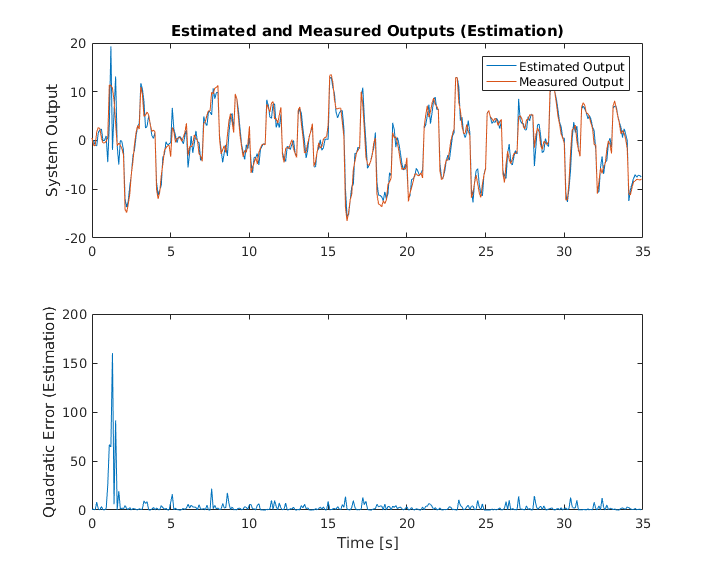
\includegraphics[keepaspectratio=true, scale=0.3]{images/arx1_performance_estimation.png}
		\caption{Performance in the estimation.}
		\label{arx1_performance_estimation}
	\end{minipage}%
	\begin{minipage}{.5\textwidth}
		\centering
		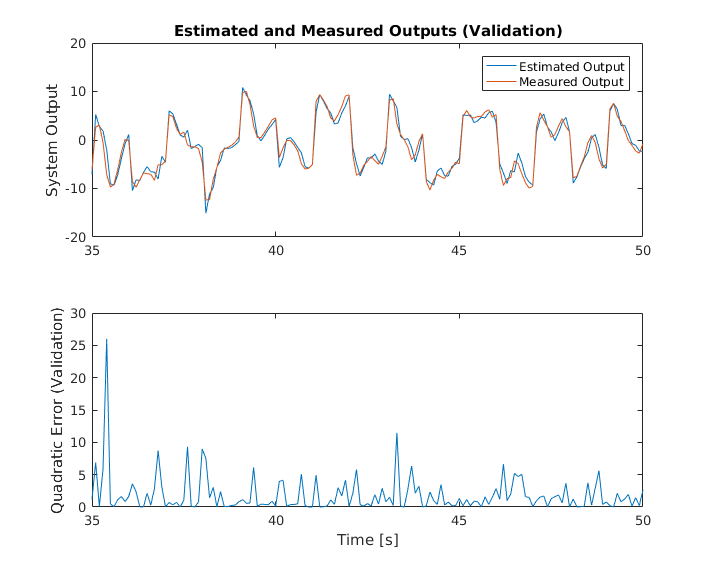
\includegraphics[keepaspectratio=true, scale=0.3]{images/arx1_performance_validation.png}
		\caption{Performance in the validation.}
		\label{arx1_performance_validation}
	\end{minipage}
\end{figure}


\subsubsection{Estimation \#2}

For the second system to estimate at this point, the $selstruct$ function produced the following values for the estimations of $n_{a}$, $n_{b}$ and $n_{k}$: $2$, $3$ and $1$, respectively.

After the on-line learning step (described in the forth step of the previous enumeration), an estimation of the \emph{ARX} model was computed, and a \emph{Mean Squared Error (MSE)} of $2.5223$ was registered over the estimation data. A fit of $65.70\%$ was also registered. Figure \ref{arx2_performance_estimation} plots the measured and estimated outputs of the system, as well as the quadratic error in the estimation process.

After the estimation process was completed, the developed estimator needed to be properly validated. In the iterative approach (using the $step$ function) a \emph{Mean Squared Error (MSE)} of $1.8668$ and a fit of $69.62$ were registered. Figure \ref{arx2_performance_validation} plots the measured and estimated outputs of the system, as well as the quadratic error in the iterative validation process. In the \emph{offline} approach, the $compare$ function yield a fit of $32.1336$.

\begin{figure}[H]
	\centering
	\begin{minipage}{.5\textwidth}
		\centering
		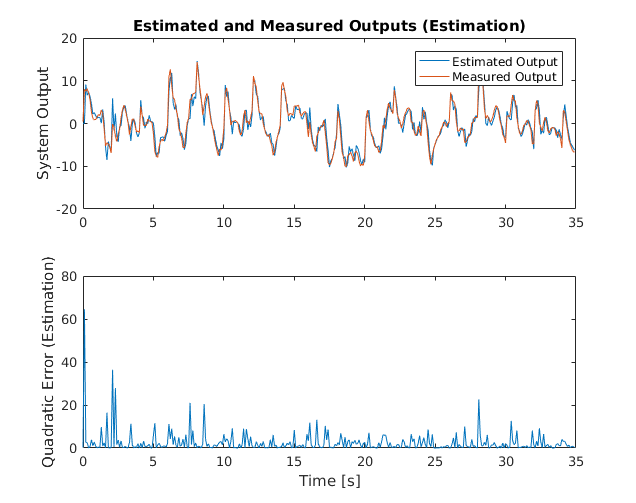
\includegraphics[keepaspectratio=true, scale=0.3]{images/arx2_performance_estimation.png}
		\caption{Performance in the estimation.}
		\label{arx2_performance_estimation}
	\end{minipage}%
	\begin{minipage}{.5\textwidth}
		\centering
		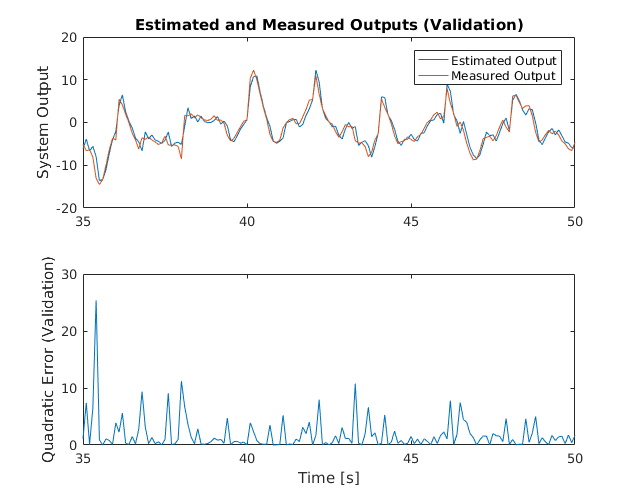
\includegraphics[keepaspectratio=true, scale=0.3]{images/arx2_performance_validation.png}
		\caption{Performance in the validation.}
		\label{arx2_performance_validation}
	\end{minipage}
\end{figure}


\subsubsection{Remarks}

Só experimentar aqui o estimador obtido para o primeiro caso no segundo e o do segundo no primeiro, e dizer que resultados é que foram observados.


\section{ARMAX Estimation}
\label{armax_estimation}

The current section covers the estimation of the parameters of the first system considered in this work, described by an \emph{ARMAX} model. Subsection \ref{theory_armax} provides a theoretical introduction to this task, while subsection \ref{parameter_estimation_armax} details the implementation.

\subsection{Theory}
\label{theory_armax}

Explicar o ARX e detalhar um pouco como funciona a estimação dos seus parâmetros

Assumir que já conhecemos a ordem

\subsection{Practice}
\label{parameter_estimation_armax}


Como nao sabemos a ordem, estimámos com o dataset, usando função blablabla.

Detalhar o dataset? - So dizer quantas observações temos e assim

Explicar os passos

\section{Conclusion}
\label{conclusion}

Comentar fit dos resultados, whatever - Comentario critico ao trabalho

\end{document}